\chapter{Detector Installation and Commissioning Organization}
\label{ch:tc-jpo}

As mentioned previously, the \dword{ipd} has responsibility for the
overall planning and execution of activities associated with component
integration and installation both in the nearby surface facilities and
underground detector caverns at \surf.  These activities are
necessarily supported by the \dword{surf} consortia who work with the
coordinators of these efforts to develop the overall plan for
assembling and installing the detectors.  The consortia are also
responsible for providing the expert personnel and specialized
equipment necessary to integrate, install and commission their
detector sub-systems.

\dword{dune} \dword{tc} provides support to the core \dword{jpo} team
responsible for installation planning and coordination.  In
particular, the coordinators and lead technicians associated with the
detector integration and installation efforts are members of the
\dword{tc} organization.  The core team also includes riggers and
other personnel responsible for the transportation and movement of
materials both to and within the \surf facility.  These team members
are associated with the \dword{sdsd}, which is responsible providing
host laboratory functions at the far site. \dword{sdsd} members of the
\dword{jpo} core team responsible for component integration and
installation include the rigging teams responsible for moving
materials in and out of the shaft, through the underground tunnels,
and within the detector caverns. \dword{sdsd} also supports team
members responsible for safety oversight and logistics planning at the
far site.

The \dword{jpo} team responsible for installation planning and
coordination is additionally responsible for the specification and
procurement of common infrastructure.  Common infrastructure includes
detector pieces such as racks, cable trays, cryostat flanges, as well
as the mechanical structure that supports the detector components from
the top of the cryostat.  It also includes general items required for
detector integration and installation such as clean rooms, cranes,
scaffolding and personnel lifts.  \dword{dune} \dword{tc} provides
engineering resources to the \dword{jpo} team to support the needed
design efforts. Specialized installation hardware associated with
specific sub-systems is provided by the consortia.


\section{Far Site Integration and Installation}
\label{sec:far_site}

All the collaboration organizations described in this chapter share
responsibilities for for far site integration and installation.
 
As mentioned in Section~\ref{sec:partners}, the \dword{ipd} 
has responsibility for the overall planning and execution of
activities associated with component integration and installation,
both in the underground detector caverns at \dword{surf} and in the
nearby surface facilities.  These activities are necessarily supported
by the \dword{dune} consortia who work with the \dword{jpo} coordinators of these
efforts to develop the overall plan for assembling and installing the
detectors.  The consortia are also responsible for providing the
expert personnel and specialized equipment necessary to integrate,
install and commission their detector subsystems.

\dword{dune} \dword{tc} provides support to the \dword{jpo} core team
that plans and coordinates installation.  In particular, the
coordinators and lead technicians associated with the detector
integration and installation effort are members of the \dword{tc}
organization.  The core team also includes riggers and other personnel
responsible for the transportation and movement of materials both to
and within the \dword{surf} facility.  These team members are
associated with the \dword{fnal} \dword{sdsd}, which is responsible
providing host laboratory functions at the far site. Under direction
of the \dword{jpo}, the underground cavern coordinator and deputy
coordinator manage the common technical resources required to
construct the cryostat, and install the cryogenics systems and
detector.


The \dword{jpo} team responsible for installation planning and
coordination is also responsible for the specification and procurement
of common infrastructure.  Common infrastructure includes detector
pieces such as racks, cable trays, cryostat flanges, as well as the
mechanical structure that supports the detector components from the
top of the cryostat.  It also includes general items required for
detector integration and installation, such as clean rooms, cranes,
scaffolding, and personnel lifts. \dword{dune} \dword{tc} provides
engineering resources to the \dword{jpo} team to support the needed
design efforts. The consortia provide specialized installation
hardware associated with specific subsystems.


\section{\dword{jpo} Management}
\label{vl:tc-facility_mgmt}

The \dword{ipd} is responsible for overall integration and
installation acitivity of \dword{lbnf} and \dword{dune} at the far
site using \dword{sdsd}. The cryostat, cryogenic and detector core
installation teams sit within the \dword{jpo}, with some members drawn
from \dword{tc}. The installation teams consist of personnel from the
consortia (e.g., students and postdocs, among others) and from
\dword{tc} (e.g., technicians and engineers). The \dword{jpo} is responsible
for coordination of activities at \surf and the \dword{ashriver} 
(shown in Fig.~\ref{fig:ash_river}).
\begin{dunefigure}[Far Site Organization Chart]{fig:ash_river}
  {Far Site Organization Chart}
  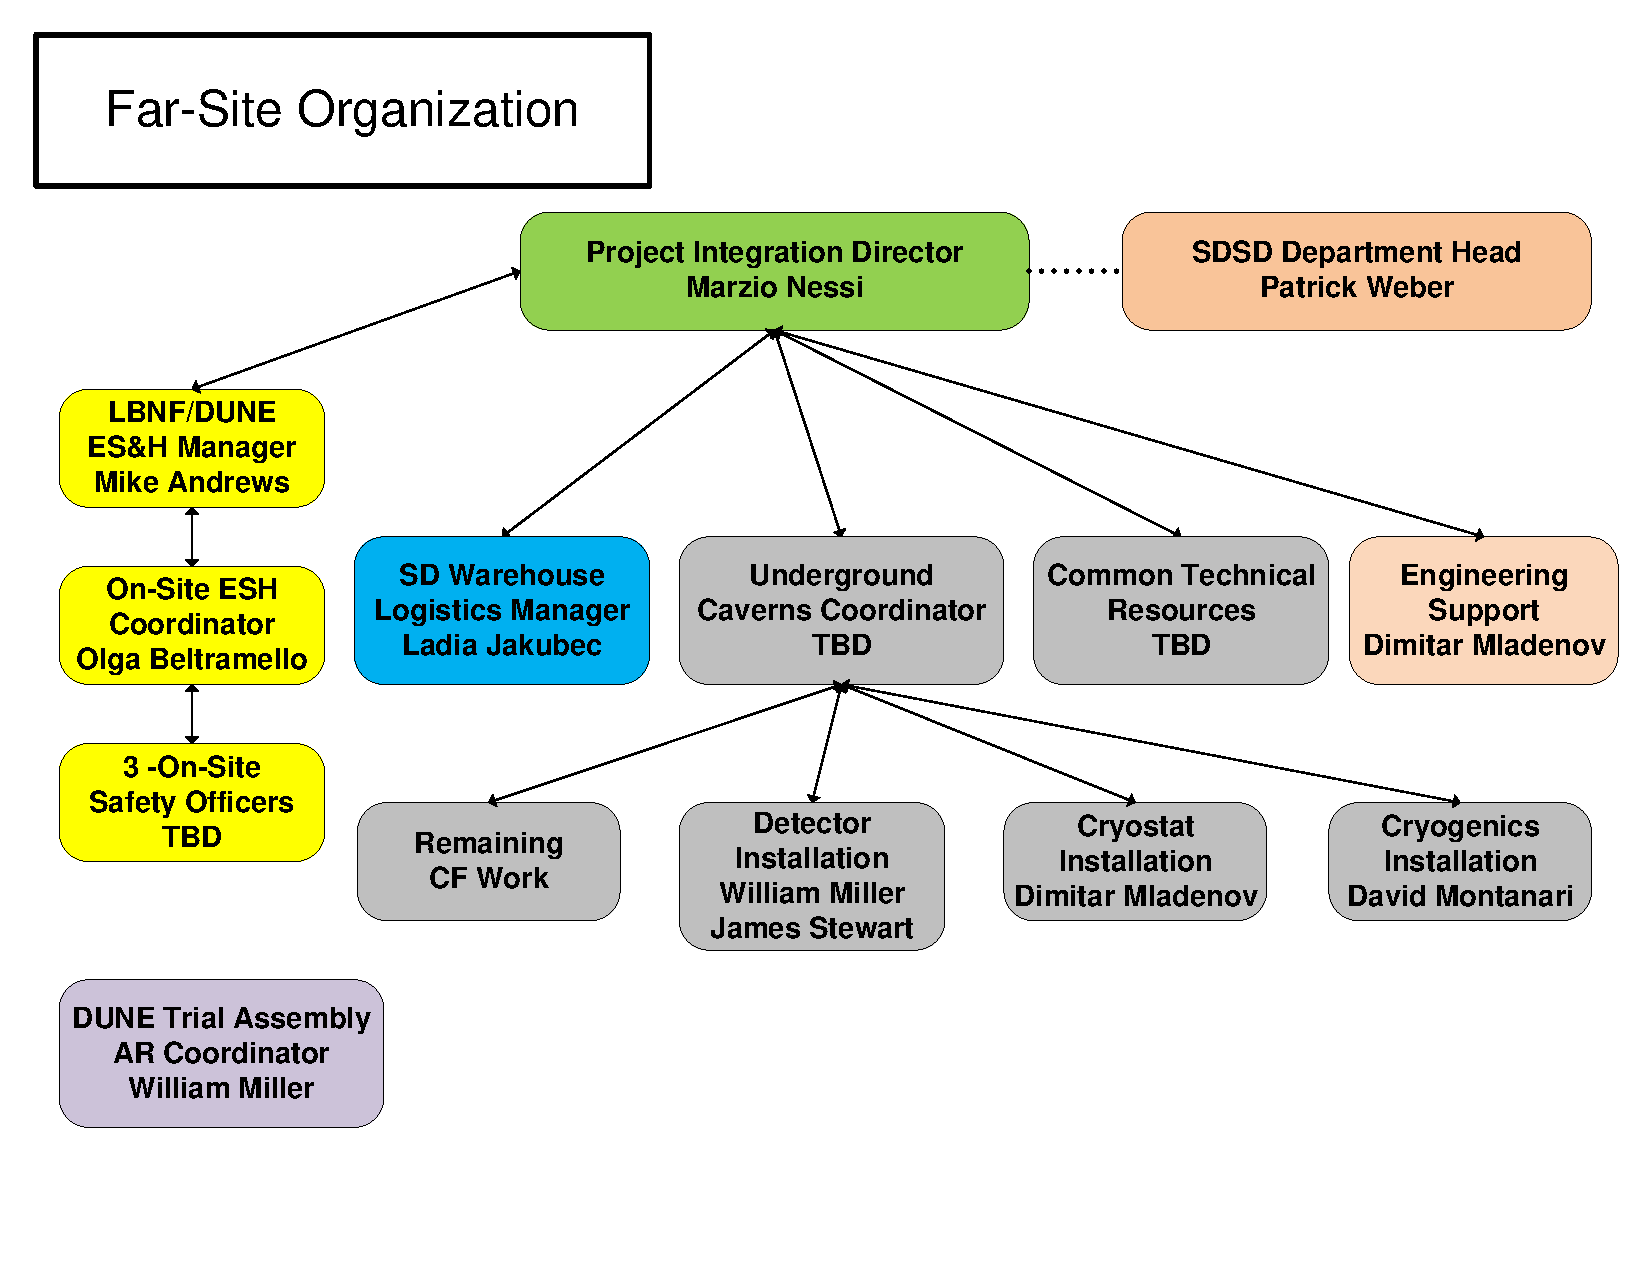
\includegraphics[width=0.95\textwidth]{Org-Far-Site-4-12-19.pdf}
\end{dunefigure}


The \dword{jpo} Management team uses the Underground Cavern Coordinator and
Deputy Coordinator to manage the technical resources required by the
five main technical resources teams:
\begin{itemize}
\item {\bf South Dakota Warehouse Facility} Receives, inventories,
  stores and delivers to the Ross headframe all the components
  delivered underground.
 \item {\bf Transport Team} Responsible for moving materials in and out
   of the shaft, through the underground tunnels, and within the
   detector caverns.
 \item {\bf Welders and Electronics Teams} Assist in the construction of
   the cryogenic infrastructure and data cable/fiber needed to operate
   the detectors
 \item {\bf Underground Integration/Installation Team} Install all the
   common infrastructure including the top and inside of the cryostat,
   plus move all the TPC components in the cleanroom and cryostat
 \item {\bf On-Call} electricians, ventilation, pluming and network
   required to keep this operating during the different phases of
   detector installation
\end{itemize}

Separately from the technical resources teams \dword{jpo} provides two
other support teams.  The safety organization headed by the
\dword{lbnf}/\dword{dune} \dword{esh} manager functions with an
onsite \dword{esh} coordinator and three onsite safety officers each
assigned to one shift.  The second is engineering support, which
includes configuration control, procurement, administrative,
mechanical and electrical engineering required for a large complex
project.

\subsection{South Dakota Warehouse Facility}

The \dword{sdwf} is a leased 5000m$^2$ facility operated by the
\dword{sdsd}.  Approximately 6 months before an \dword{aup} is given
the \dword{sdwf} is needed to receive the components of warm structure
and the \dword{apa} shipping frames. Laydown space near the Ross
headframe is extremely limited; therefore, careful coordination of
shipments to the Ross shaft is required. The \dword{lbnf} logistics
manager is responsible to coordinate shipments underground with the
\dword{cmgc} and \dword{jpo}. Since no materials or equipment may be
shipped directly to the Ross or Yates headframe, the \dword{sdwf} is
used for both short and long-term storage and re-packaging before
anything is shipped underground. The function of the \dword{sdwf}
shown in Fig.~\ref{fig:sdwf} incudes the coordination between the
underground caverns coordinator, the logistics manager and the
installation teams needing materials underground.
\begin{dunefigure}[South Dakota Warehouse Facility team]{fig:sdwf}
  {South Dakota Warehouse Facility team}
  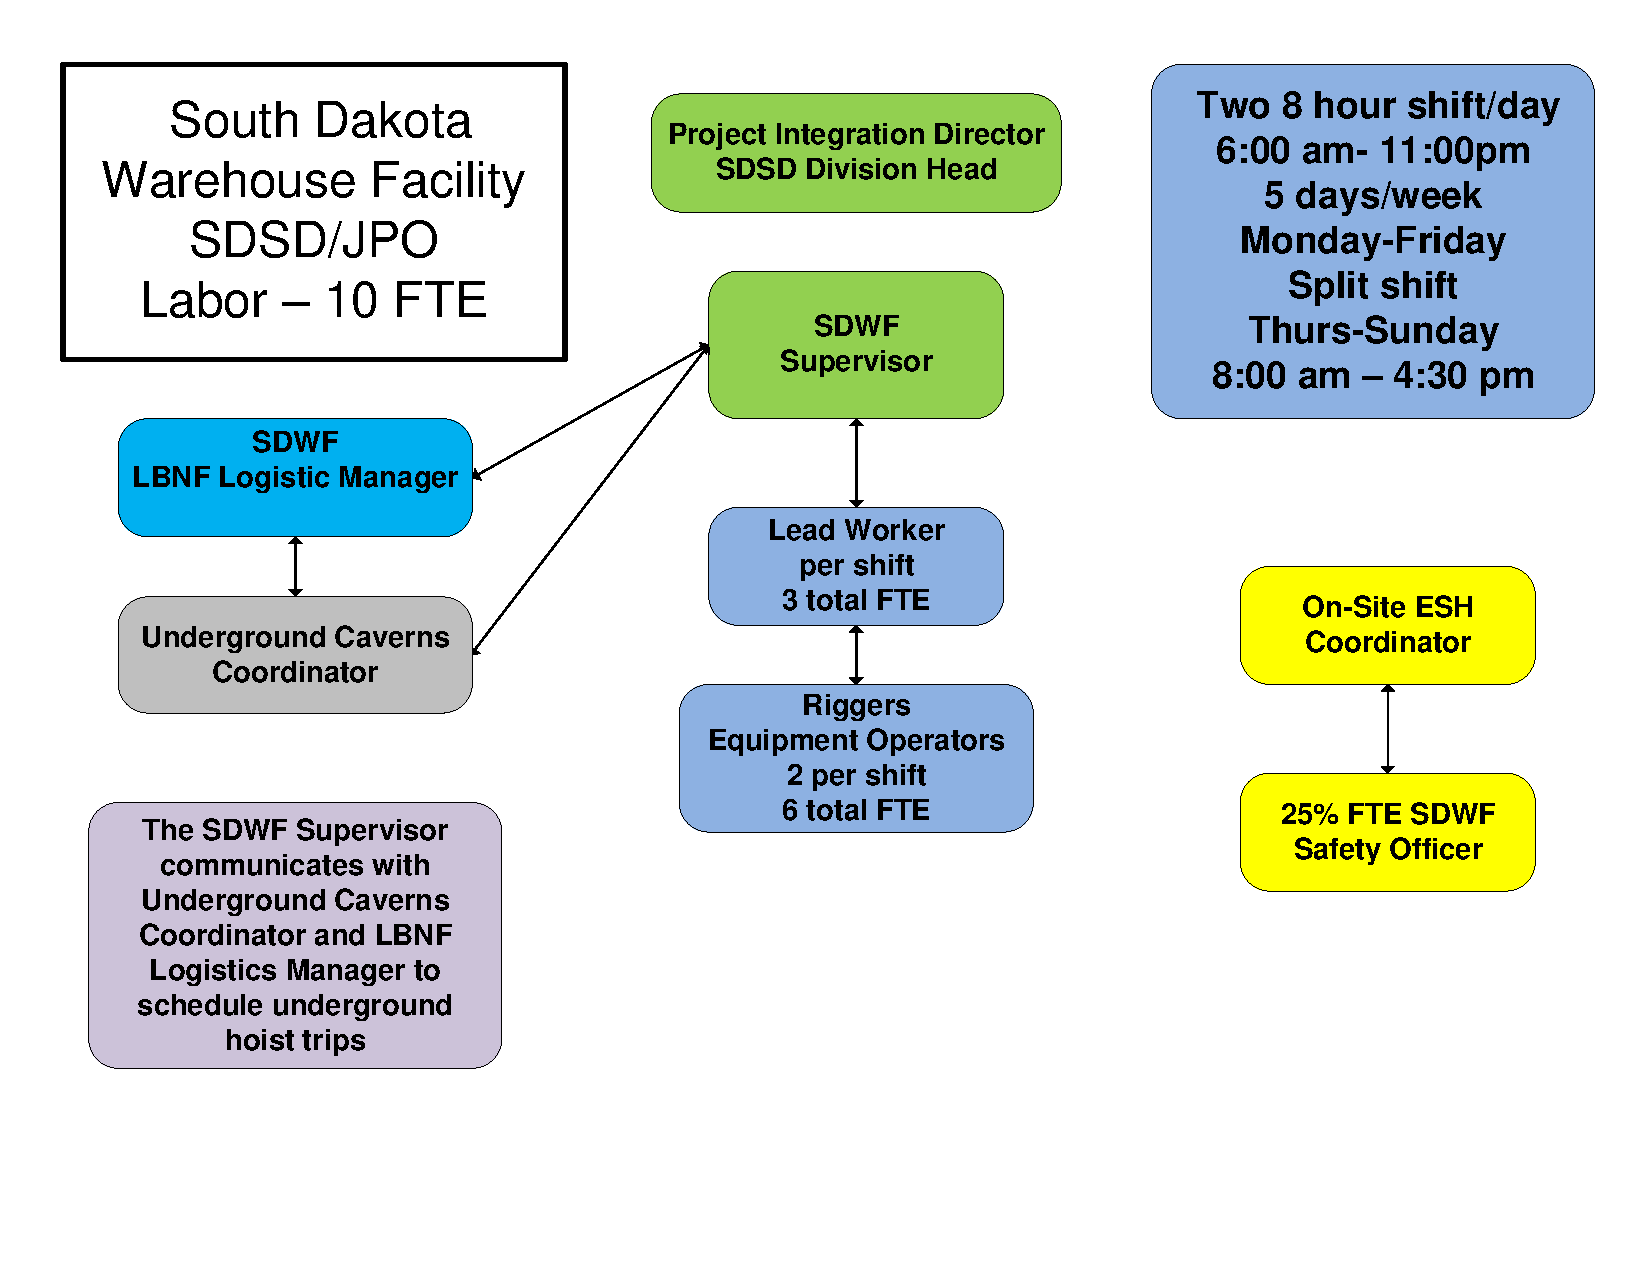
\includegraphics[width=0.95\textwidth]{Org_SDWF-4-5-19v2.pdf}
\end{dunefigure}

The \dword{sdwf} is operated seven days per week, with two shifts per
day Monday thru Friday and a split shift day shift on the weekend
since access underground is 24/7. The facility is managed by the
\dword{sdwf} supervisor with three lead workers with a small
\dword{jpo} crew of professionally trained riggers/equipment operators
to operate 16 hours/day Monday--Friday and a split day shift to cover
the weekends.  There is also a small team (one FTE/shift) provided by
the consortia using the inventory system to track all materials coming
in and out of the \dword{sdwf}. Some repackaging will be required to
fit materials in the cage or on a slung load.  Management must work
directly with the \dword{lbnf} logistics team at \surf and the
\dword{cmgc} so that loads to the headframe arrive as scheduled. The
headframe has room for only 1--2 trucks, so proper scheduling is
critical.

The part time safety officer is shared with the \dword{uit} under the
direction of the onSite \dword{esh} coordinator.  The safety officer has
several responsibilities, insuring that all the \dword{sdwf} personnel are
properly trained, all safety documentation and procedures are up to
date and stored on \dword{edms} and participating in the daily/weekly toolbox
meetings when needed.

\subsection{Underground Facilities}


There are three main phases of the underground work once \dword{aup}
of the north cavern and \dword{cuc} are given shown in
Fig.~\ref{fig:underground_schedule}:
\begin{itemize}
 \item {\bf Cryostat construction} --- Warm and Cold structure
 \item {\bf Central Utility Cavern} --- DAQ Infrastructure, control room
   and cryogenics installation
 \item {\bf Detector Integration/Installation} --- Cleanroom, installation
   infrastructure and TPC component installation inside the cryostat.
\end{itemize}
\begin{dunefigure}[Underground summary schedule]{fig:underground_schedule}
  {Summary schedule or the different phases of work underground}
  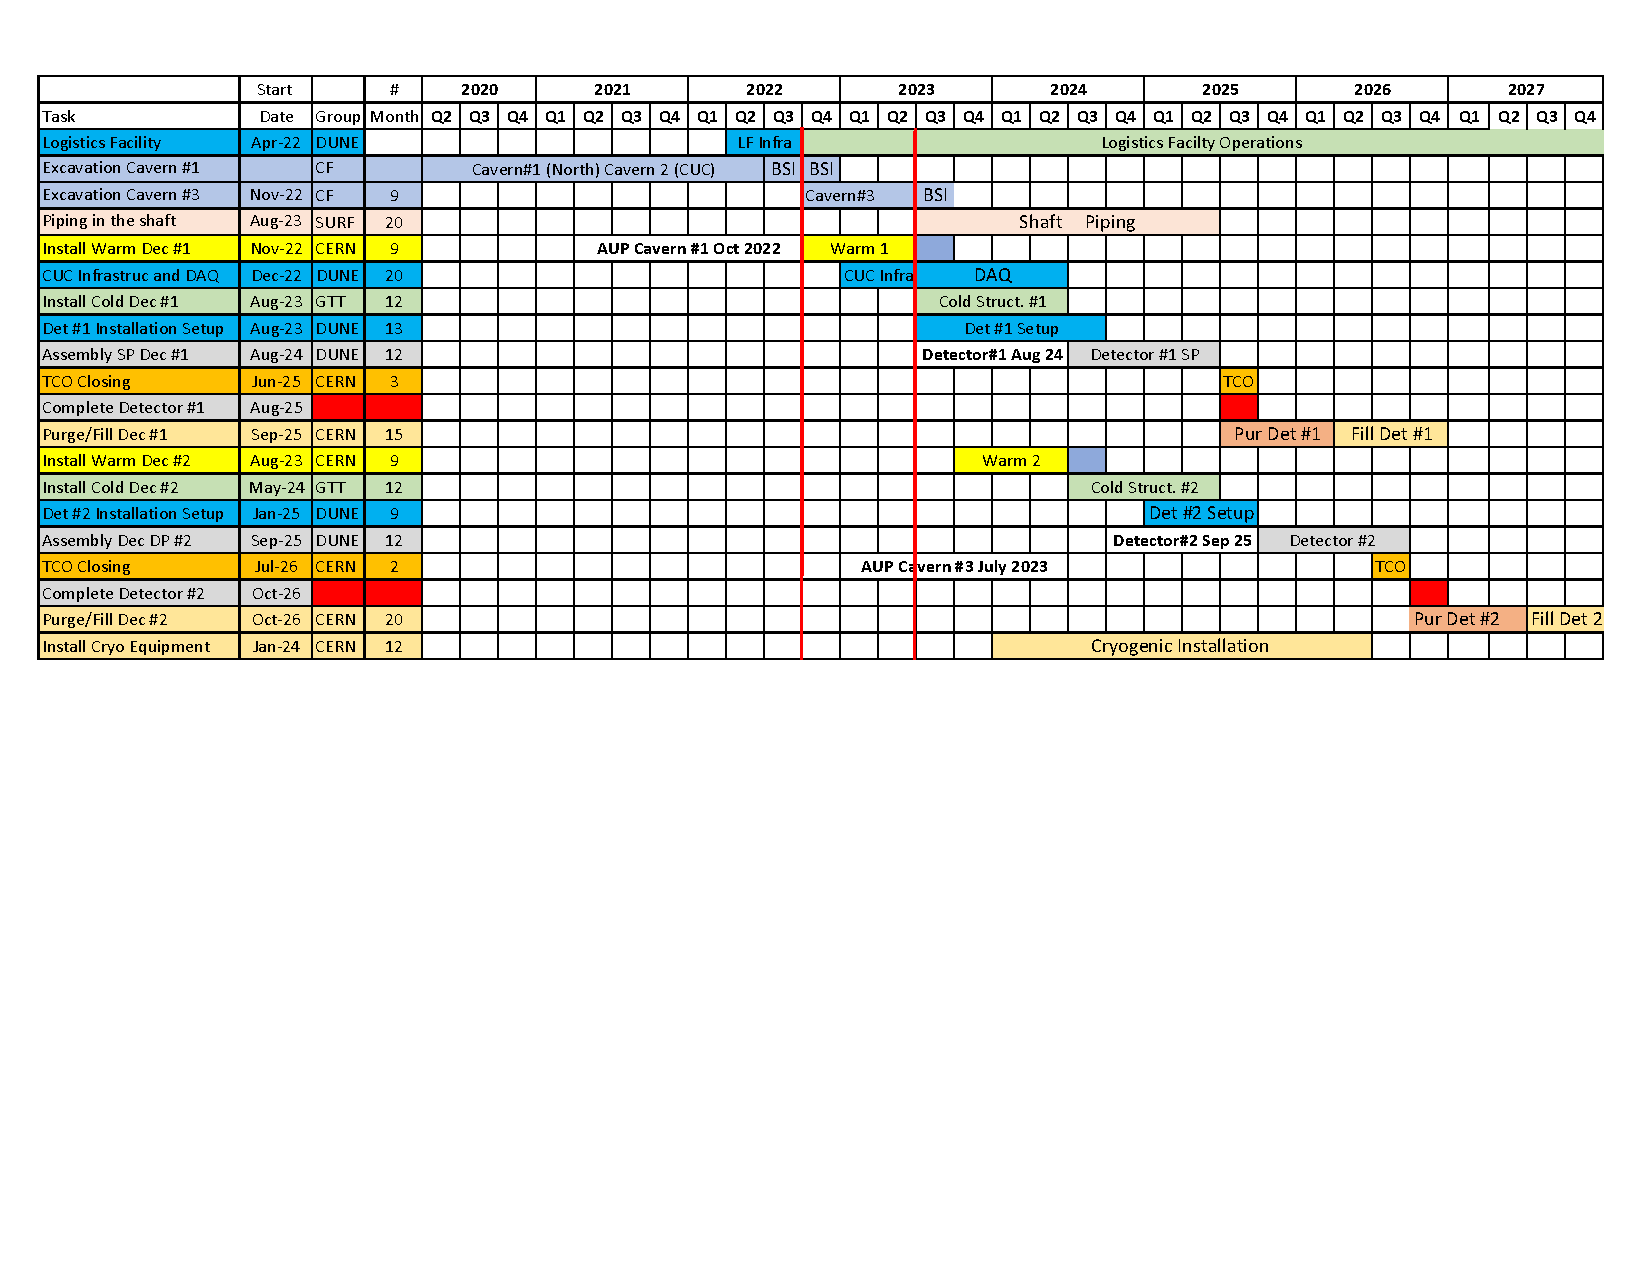
\includegraphics[width=0.85\textwidth]{Summary_Schedule.pdf}
\end{dunefigure}


The schedule depends on critical cooperation between CF, \dword{lbnf}
and \dword{jpo} to control the limited number of FTE underground and
hoist access.  This is especially difficult while CF is completing the
excavation and BSI work on the South Cavern.  \dword{jpo},
\dword{sdsd}, \dword{lbnf} and CF will minimize interference and
maximize efficiency by managing adjustments to this schedule.  The
size of the Technical Resources will increase during the early stages
and help train key managers and lead workers as we move into detector
integration/installation.  Figure~\ref{fig:ctr_orgchart} shows the
management structure of the Common Technical Resources labor force of
57 FTE.
\begin{dunefigure}[Common Technical Resources]{fig:ctr_orgchart}
  {Summary of the \dword{jpo}/\dword{sdsd} Common Technical Resources}
  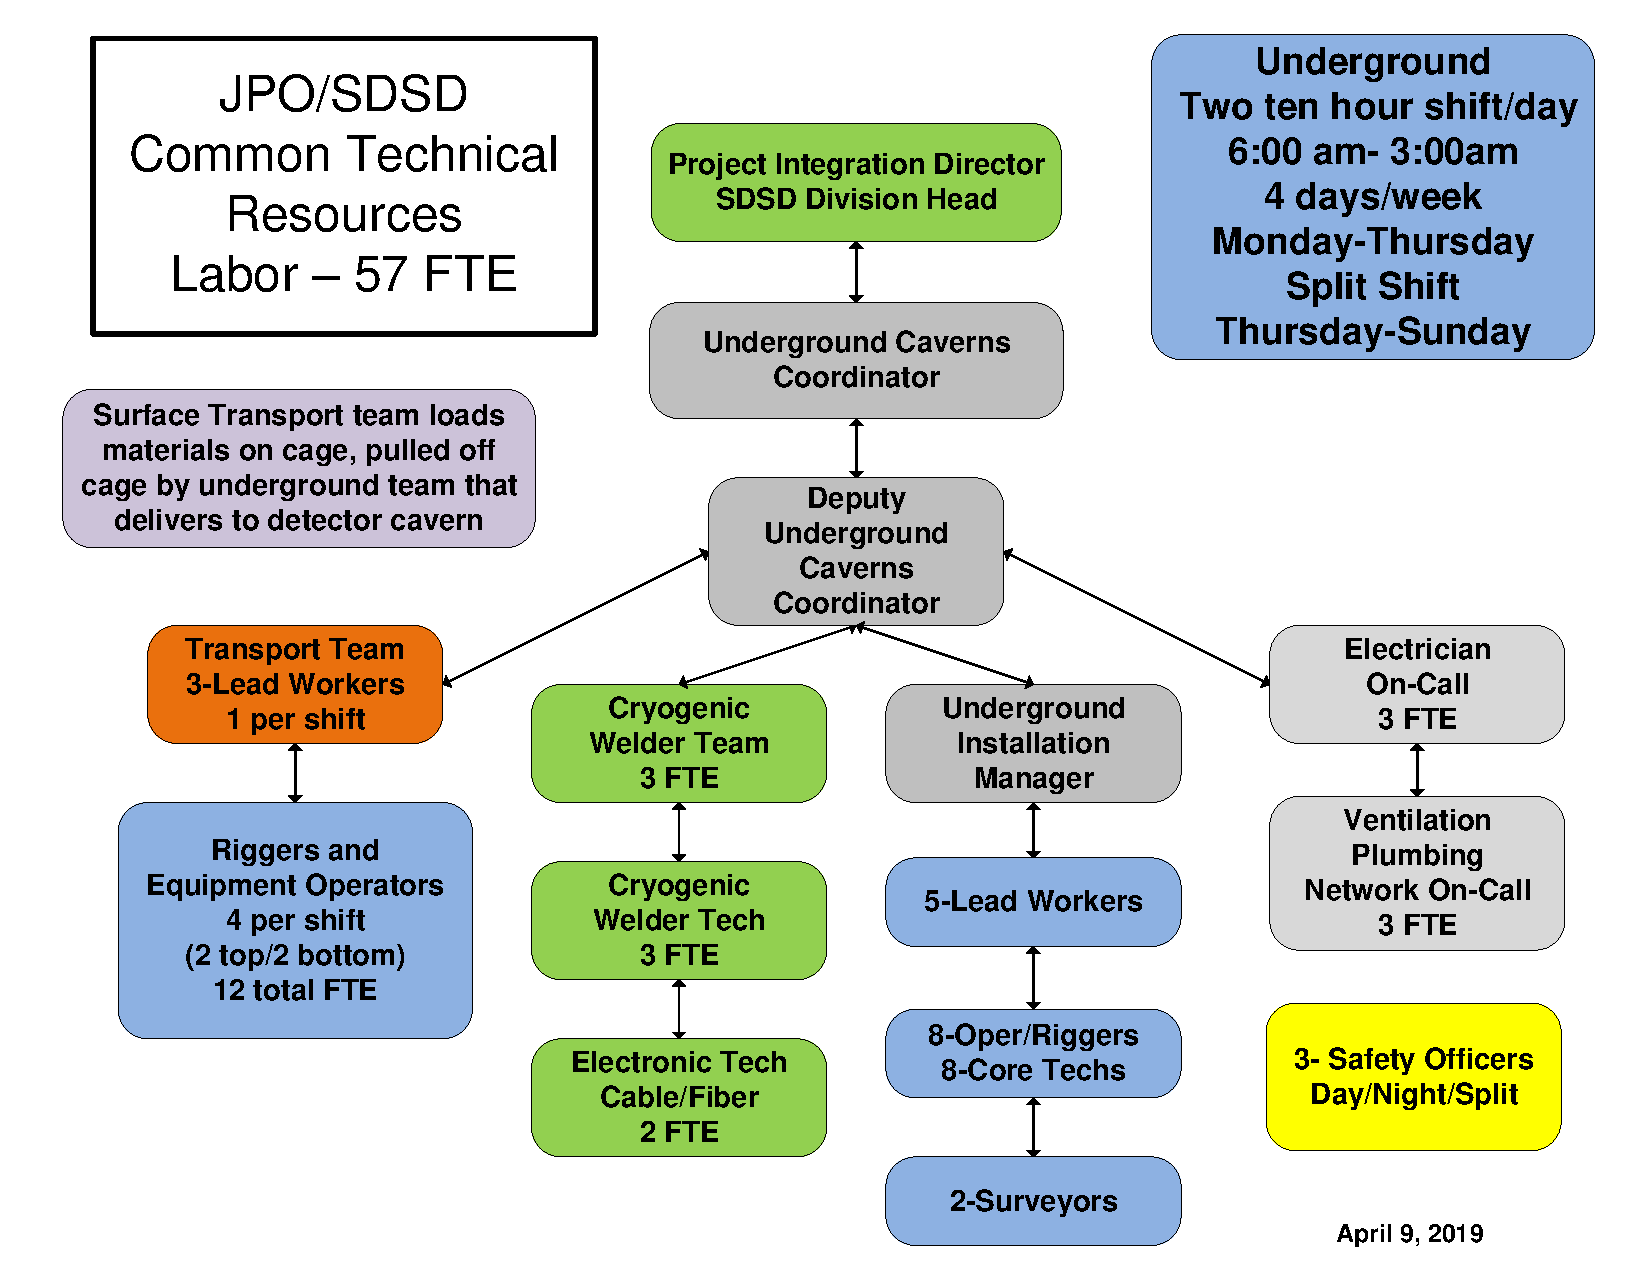
\includegraphics[width=0.95\textwidth]{Org_Technical_Resources-JPO-4-9-19.pdf}
\end{dunefigure}

The responsibilities of the Underground Cavern Coordinator and common
technical resources is complex because of the material movement
involved getting components and equipment a mile underground then to
the proper location the cleanroom and cryostat:
\begin{itemize}
  \item {\bf Transport team} --- Unload materials from the trucks arriving
    from the \dword{sdwf}, load them into the cage in the Ross Shaft on the
    surface and unload them at the shaft station on the 4850 level.
    They then deliver the components to the correct location in the
    \dword{dune} complex.
  \item {\bf \dword{uit} Riggers/Core Techs}
    \begin{itemize}
      \item North, Central and South Caverns --- Cryostat, cryogenic,
        TPC components and infrastructure materials can be stored in
        the available cavern space during the construction of
        detectors \#1--2.  The \dword{uit} riggers/core techs team will use
        forklifts, carts and cavern crane to move materials into the
        clean room.
      \item Inside the SAS and clean room: The main tasks are
        manipulating \dwords{apa} onto the different \dword{apa}
        towers and \dword{cpa} component assembly. The team operates
        the shuttle beam and crane, opens and closes the cold boxes
        and moves materials with forklift, carts and motorized pallet
        jacks.
      \item Inside the Cryostat: The \dword{uit} team installs the
        \dword{dss} and cryostat subfloor; they then move the
        completed \dword{apa} and \dword{cpa} pairs into
        position. They also deploy the \dword{fc}.
    \end{itemize}
  \item {\bf On-call Electricians, Ventilation, Plumbing and Network
    team}--- As the different phases of the \dword{lbnf}/\dword{dune}
    construction progress an on-call team of contractors will be
    required to modify systems as they change after CF has completed
    the initial stage.
   \item {\bf Cryogenic Welders, Technicians, Electronic technicians and Surveyors}
\end{itemize}

These teams including consortia working underground typically work
four 10-hour day and afternoon shifts.  A day split shift covers
Thursday--Sunday. This is needed when the hoist is available to hauling
materials underground and to oversee APAs in the cold box over the
weekend.

On the surface at the start of each shift, there is a daily toolbox
safety meeting and work assignment update. An hour separates the two
shifts to allow the lead workers, safety officer and management would
have overlapping shifts to insure proper transfer of knowledge. The
safety officer on each shift would be responsible for any discussion
of safety during the meeting but also for training all workers,
including those from the consortia.  The safety officer management
goes directly to the \dword{lbnf}/\dword{dune} \dword{esh} manager to
minimize any conflict of interest although all \dword{uit} and
consortia personnel have the right to stop work for any safety issues.

The \dword{uit} is responsible for the integration and installation of
the \dword{dune} detectors.  The management not only supervises the
technical resources but also works the consortia teams to maximize the
efficiency of the installation process. Figure~\ref{fig:uit_orgchart}
shows the management and labor force working in the cleanroom and
cryostat.
\begin{dunefigure}[\dword{uit}]{fig:uit_orgchart}
  {The Underground Detector Integration/Installation Team}
  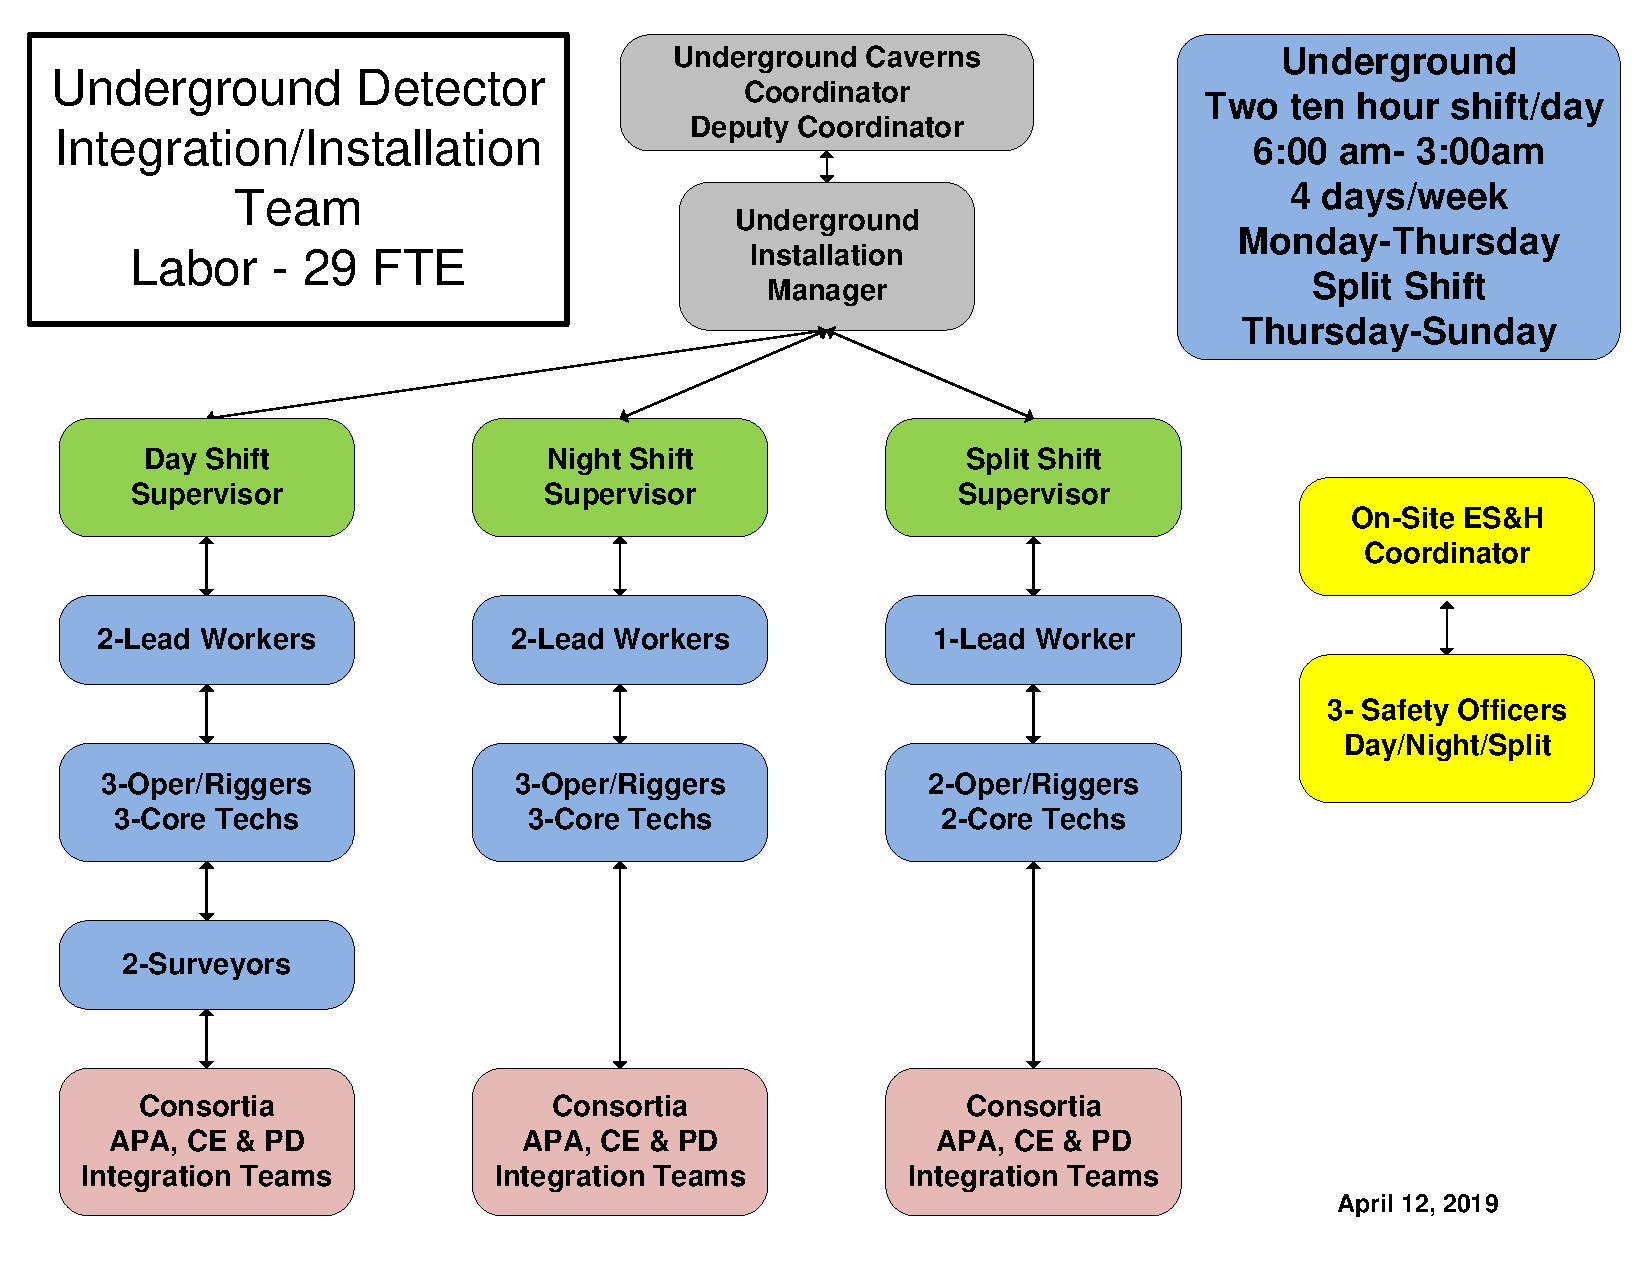
\includegraphics[width=0.95\textwidth]{Org_UIT-4-12-19.pdf}
\end{dunefigure}
Underground Detector Integration/Installation Team management consists
of three levels:
\begin{itemize}
  \item {\bf Underground Installation Manager:} The \dword{uit} manager oversees
    both shifts but also covers for the day or night shift deputy
    manager if needed. This \dword{uit} manager is the contact person working
    directly with the Underground Caverns Coordinator to organize cage
    trips for materials needed underground, attending all high-level
    meetings as required, and submitting weekly progress reports. The
    \dword{uit} manager schedules and organizes the work along with the
    consortia to ensure they have the rigging crews at the appropriate
    times.
  \item {\bf Day/Night/Split shift Installation Supervisors:} The deputy
    supervisors are working managers, trained riggers and equipment
    operators who can fill in as needed. They are trained in all
    installation procedures, working directly with the consortia to
    keep the project on schedule. If the lead worker is sick or on
    vacation, the installation shift supervisors fill
    in. Communication among the installation shift supervisors between
    shifts is critical for a smooth shift change.
  \item {\bf Lead Workers:} The lead workers typically are the main
    equipment operators and direct the individual teams, which
    typically comprise 2--3 riggers or equipment operators. The lead
    workers are trained in all installation procedures and help the
    consortia as needed for each task.
\end{itemize}
        

\subsection{Ash River}

Ash River is the site of the NOvA far detector in Ash River,
Minnesota. The NOvA far site detector hall offers a \SI{16.75}{m} deep
pit with $\sim$\SI{300}{m$^2$} of floor space available for testing
DUNE detector components at full scale.  The trial assembly work at
Ash River has three major phases of \dword{dune} mechanical tests to
confirm designs and practice installation techniques, including design
modifications from \dword{protodune}.  The \dword{nova} Far Detector
Laboratory is managed by the University of Minnesota and is partially
funded through an operations grant from Fermilab.  Work follows both
university and Fermilab safety regulations, whichever is more
stringent. University code officials approve all building
permits, which include engineered drawings signed by an engineer
registered in Minnesota. All hazard analyses and work procedure
documents are approved by a joint safety committee with members drawn
from both the University of Minnesota and Fermilab and may include
specialists as needed.

The work at Ash River has four main goals:
\begin{itemize}
  \item Verify that the \dword{dune} \dword{tpc} can be installed as
    safely and efficiently as possible
  \item Use the \dword{protodune} Trial Assembly \dword{dss} to test
    mechanical design changes for \dword{protodune2}
  \item Complete a set of procedural documents as the basis for work
    underground at \surf
  \item Serve as a training center for \dword{dune} integration and
      installation for new hires at \surf
\end{itemize}

There is a full time staff of five \dwords{fte} at Ash River. A
manager, deputy manager and three experienced technicians.  One of the
technicians is also the safety officer and chairperson of the joint
safety committee. The staff size will be increased by two FTE with the
additional workload of \dword{protodune2}.

{\bf Phase 0:} A vertical cable test of two full-scale \dword{apa}
side tubes have been mounted to a column in the lab for cable tests
and the \dword{protodune} Trial Assembly Frame continues to be used
for \dword{protodune2} mechanical tests. Using complete cable
bundles we have tested how well the conduit system works and several
possible modifications. We have completed a series of tests for
mounting the \dword{gp} or \dword{protodune2} and started the first
full scale mechanical \dword{fc} test with the new design.


{\bf Phase 1:} We have constructed a prototype of the \dword{dune} \dword{apa} tower
using a steel frame large enough to hold a commercial stair scaffold
in the middle as shown in Figure~\ref{fig:ashriver1}.
\begin{dunefigure}[3-D model of the APA Tower at Ash River]{fig:ashriver1}
  {3D model of the Phase 1 Trial Assembly \dword{apa} Tower at the NOvA Far Detector
    Lab in Ash River.}
  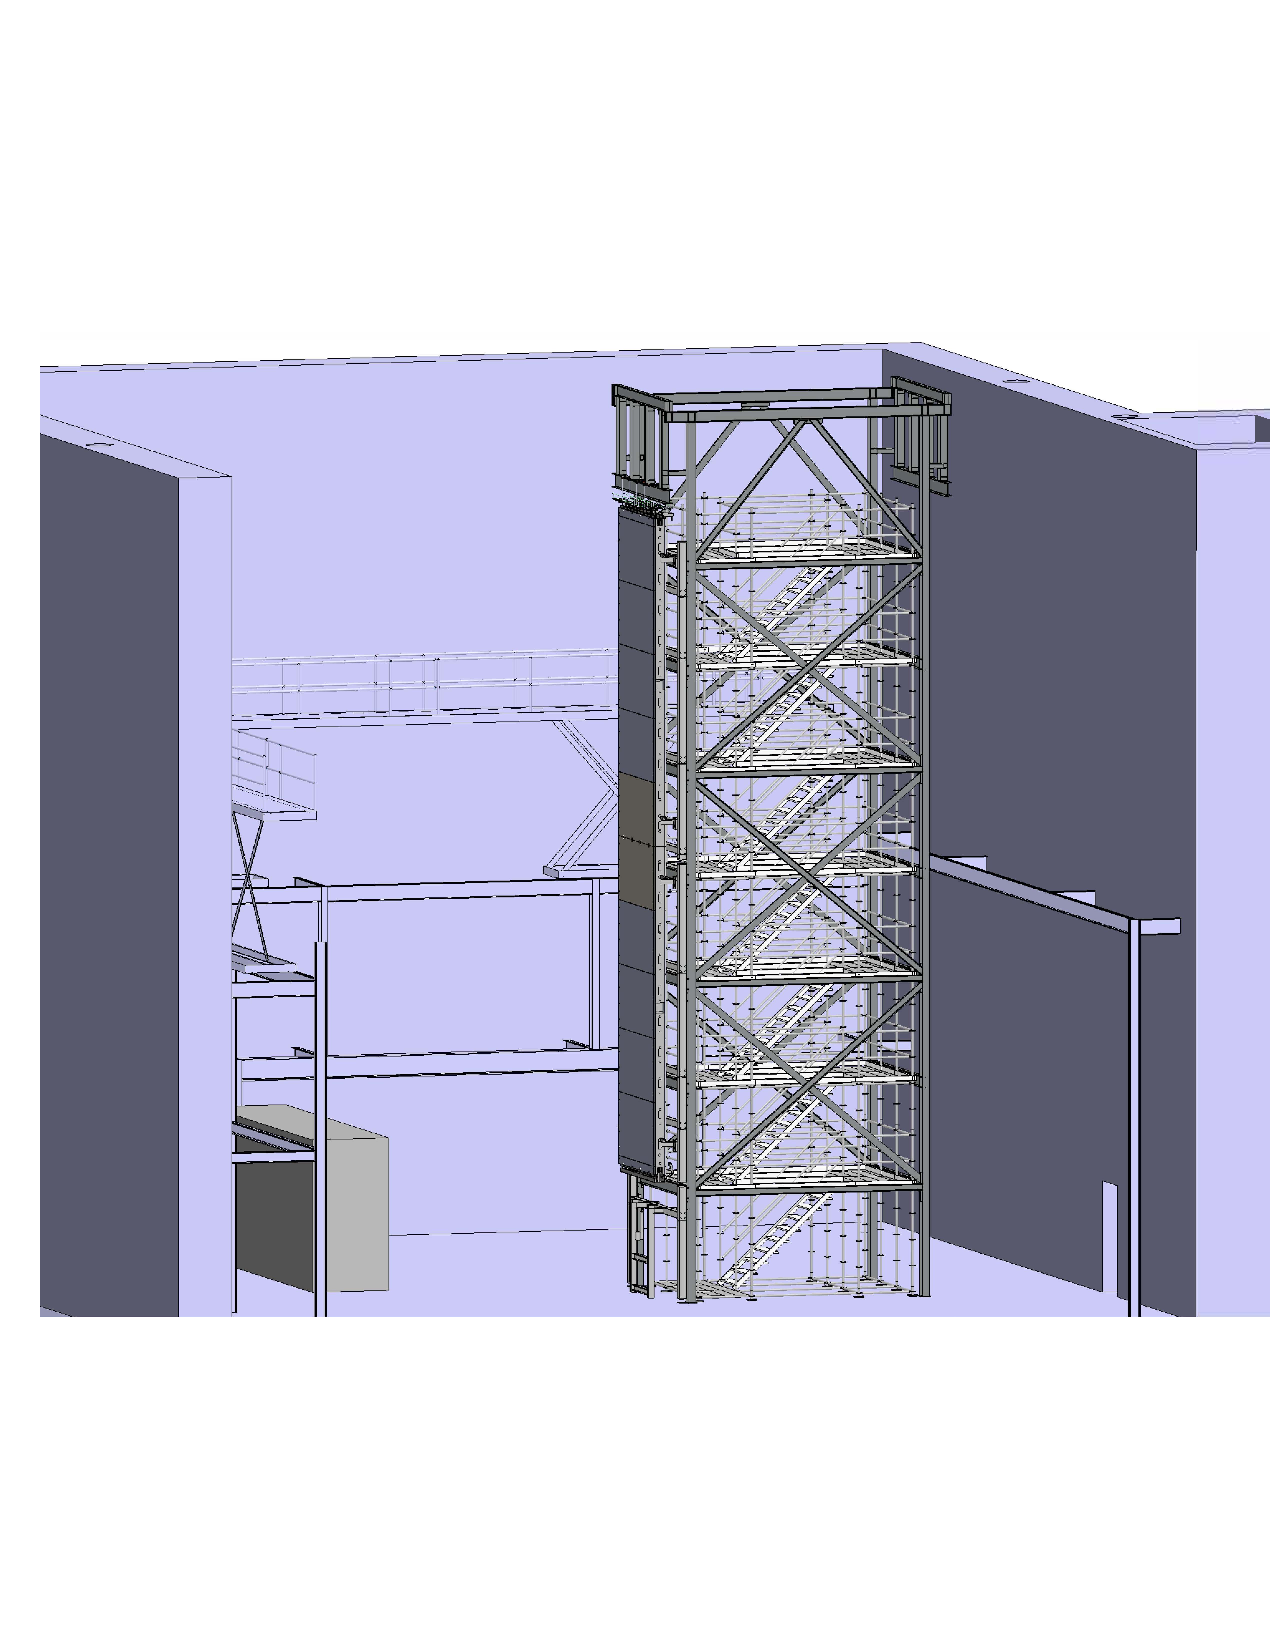
\includegraphics[width=0.65\textwidth]{APA_Tower_at_AshRiver.pdf}
\end{dunefigure}
This \dword{apa} tower is designed so we can use it for joining the
top and bottom \dword{apa} together and test all the cabling
procedures.  This tower will allow us to test all mechanical
integration/installation tests for the \dword{apa} doublet. In the
fall of 2019, we will add a \dword{cpa} assembly station and test the
new \dword{cpa} assembly procedures.  Also planned is a prototype
\dword{apa} shipping frame to test the many features of the shipping
container.

{\bf Phase 2:} In FY20, a more complex steel structure will be
constructed. It is designed to mock up several sections of the
\dword{dss}. This allows a complete full-scale mechanical assembly of
the TPC components as seen in Figure~\ref{fig:ashriver2}.
\begin{dunefigure}[Phase 2 Trial Assembly at Ash River]{fig:ashriver2}
  {Phase 2 Trial Assembly at Ash River}
  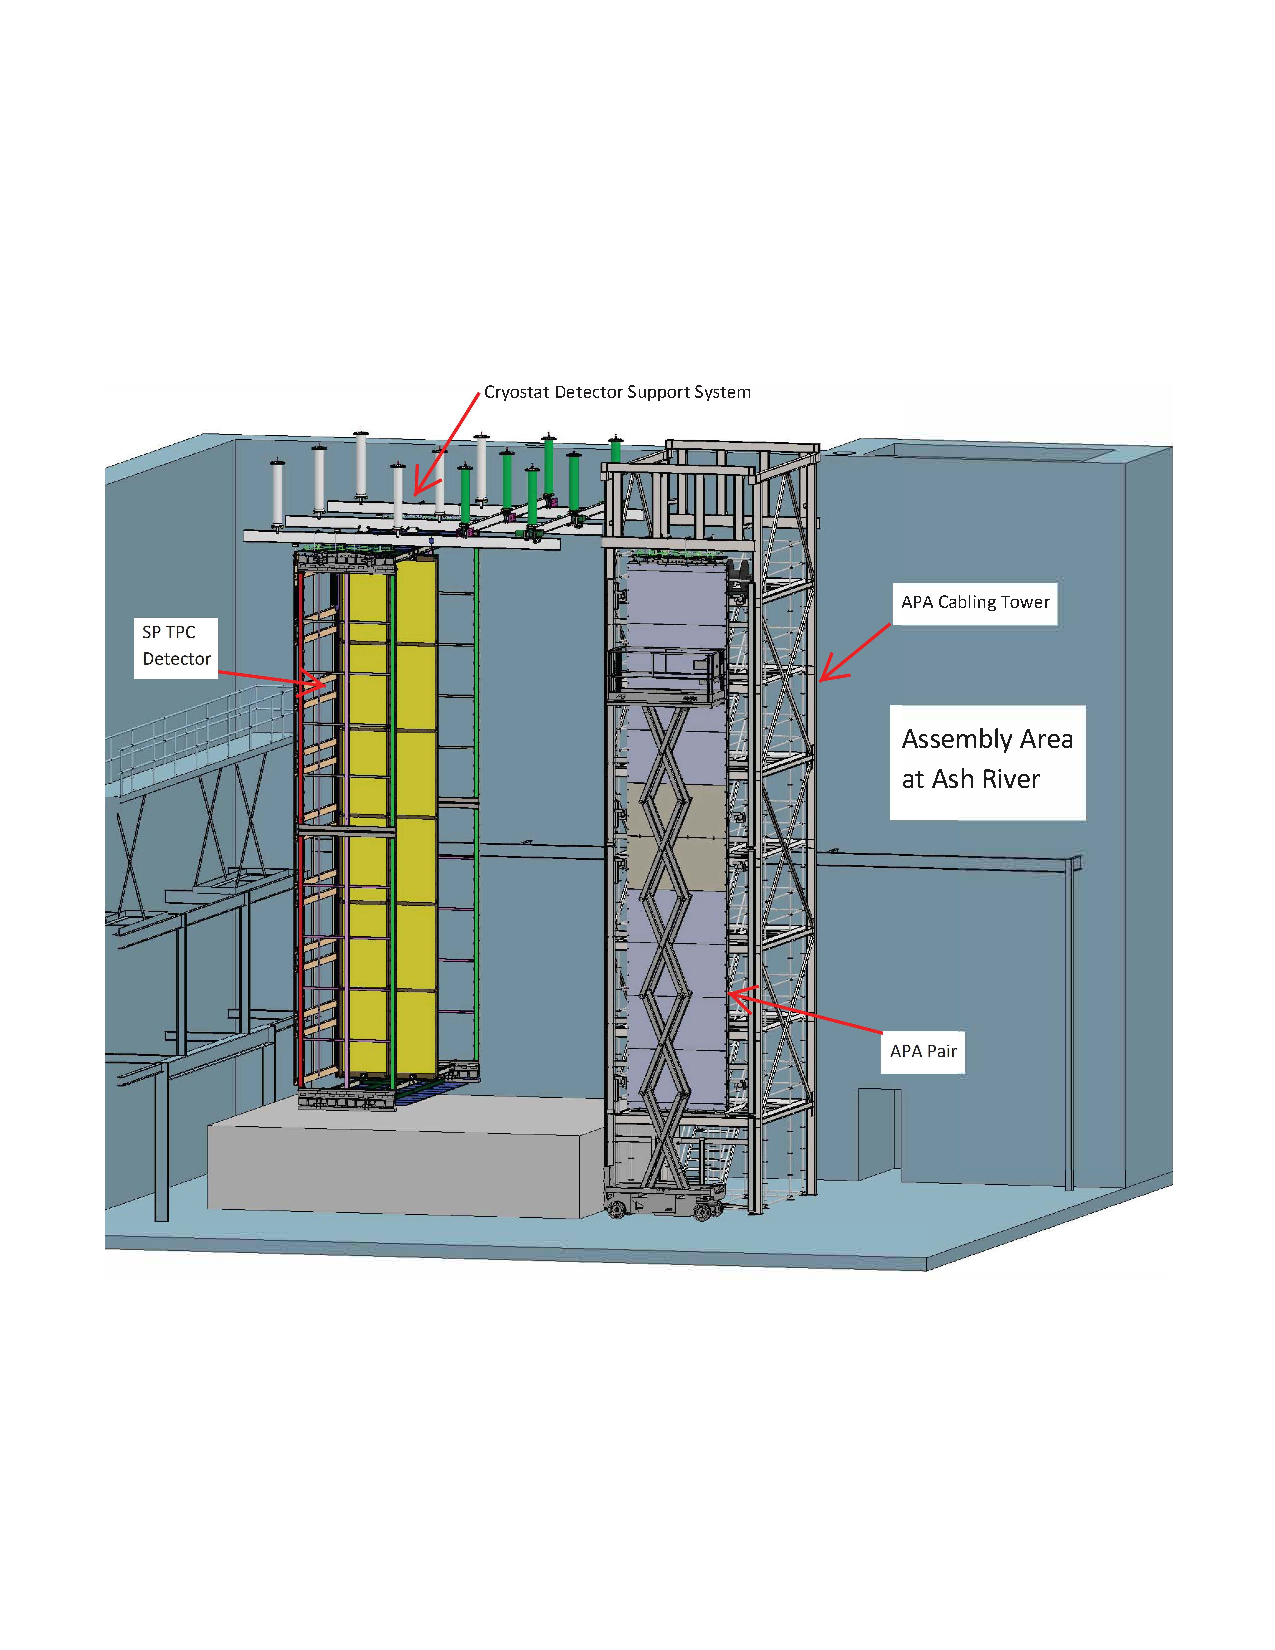
\includegraphics[width=0.65\textwidth]{Phase2_Trial_Assembly.pdf}
\end{dunefigure}
This facility enables tests of procedures using this structure including:
\begin{itemize}
 \item Installation of the \dword{dss}
 \item Transfer of TPC component through the \dword{tco}
 \item Installation of the end walls
 \item Cabling of the \dword{apa} through the cryostat penetrations
 \item Moving \dword{apa} and \dword{cpa} pairs into final position and deploying the field cages
 \item Deployment of the Dual Phase detector
\end{itemize}

\section{\dword{dune} Host Facility Services}
\label{sec:fdsp-coord-host_facility_services}

This section is under development. The plan is to ask Patrick to write
it.

The intent of this section is to describe the services that are
provided by the host facility.

The following is preliminary outline, there may already be a document
with a more comprehensive plan.
\begin{itemize}
\item Detector component transportation to underground cavern and rigging
\item Removal of equipment packaging from undergoing cavern
\item Electical and plumbing contracted services
\item Maintenance and readiness of lifts, moving equipment and associated items
\item Maintenance and operation of cooling water systems for detector and CUC
\item Maintenance and operation of networking equipment
\item Maintenance and operation of electrical installations for detector power
\item Building and cavern services such as lighting, air handling and
  filtration, fire safety and suppression, safety rails, dew point
  control, hazard alarms (fire and ODH)
\item Hazard awareness and safety training
\item Storage areas for tools and PPE
\item Facility life saftey systems
\item Plan for medical emergencies and medical evacuation
\item Underground emergency plans and procedures
\item Controlled access plan and equipment
\item Maintenance of ground impedance monitors and detector ground Isolation
\end{itemize}


Resources for the personnel and activities associated with \dword{tc}
are provided through a mixture of common collaboration funds and
support from the host nation.  During the construction phase of the
experiment, \dword{dune} will collect an annual membership fee from
each Ph.D. scientist within the collaboration.  The collected funds
will be used primarily for supporting the personnel included within
the \dword{tc} team.  Funding agencies will have the option of
directly providing team members in lieu of cash contributions.

The acquisition of common infrastructure will be supported through
additional collaboration common funds collected from the funding
agencies as a percentage of the value of their contributed detector
deliverables.  As in the case above, funding agencies will be given
the option of directly providing equivalently valued infrastructure
items as opposed to actual cash contributions.  Host Laboratory
functions provided by the \dword{sdsd} will be supported directly host
nation funding agency \dword{doe}.

All project partners will sign an MOU that specifies which detector
deliverables will be provided by each of the supporting funding
agencies.  The MOU will also specify the required common fund
contributions from each of the participating funding agencies.  The
DUNE resource coordinator will be responsible for managing and
reporting on all common fund contributions.
